\section{Identifier}
\label{sec:Identifier}
%%%%%%%%%%%%%%%%%%%%%%%%%%%%%%%%%%%%%%%%%%%%%%%%%%%%%%%%
\begin{figure}[h!]
\begin{center}
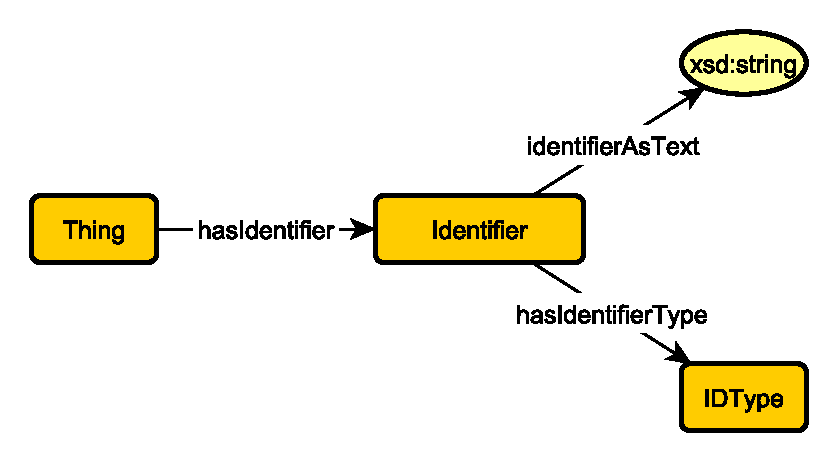
\includegraphics[width=.7\textwidth]{figures/identifier}
\end{center}
\caption{Schema Diagram for the Identifier Pattern. The visual notation is explained in Chapter \ref{chap:prelims}.}
\label{fig:Identifier}
\end{figure}
\subsection{Summary}
\label{sum:Identifier}
%%%%%%%%%%%%%%%%%%%%%%%%%%%%
This pattern is used for associating some sort of identifier and metadata with a thing. One could view this pattern as a reification of the \textsf{ExplicitType} Pattern as found in Section \ref{sec:Explicit}. In this case, we wish to associate additional information aside from its type with a thing, e.g. an identifier may be a URL or a primary key value in a database. We believe that this pattern meshes well with the \textsf{EntityWithProvenance} Pattern which may be found in Section \ref{sec:Provenance}.

%%%%%%%%%%%%%%%%%%%%%%%%%%%%%%%%%%%%%%%%%%%%%%%%%%%%%%%%
\subsection{Axiomatization}
\label{axs:Identifier}
%%%%%%%%%%%%%%%%%%%%%%%%%%%%
\begin{align}
% General Axioms
% Domain and Range restrictions
\top &\sqsubseteq \forall \textsf{hasIdentifier.Identifier} \\
\exists \textsf{hasIdentifierType.}\top &\sqsubseteq \textsf{Identifier} \\
\top &\sqsubseteq \forall \textsf{hasIdentifierType.IDType} \\
\top &\sqsubseteq \forall \textsf{identifierAsText.xsd:string}
% Inverse Aliases (if any)
\end{align}

%%%%%%%%%%%%%%%%%%%%%%%%%%%%%%%%%%%%%%%%%%%%%%%%%%%%%%%%
\subsection{Explanations}
\label{exp:Identifier}
%%%%%%%%%%%%%%%%%%%%%%%%%%%%
\begin{enumerate}
\item Range: the range of \textsf{hasIdentifier} is \textsf{Identifier}.
\item Domain: the domain of \textsf{hasIdentifierType} is \textsf{Identifier}.
\item Range: the range of \textsf{hasIdentifierType} is \textsf{IDType}.
\item Range: the range of \textsf{identifierAsText} is \textsf{xsd:string}.
\end{enumerate}

%%%%%%%%%%%%%%%%%%%%%%%%%%%%%%%%%%%%%%%%%%%%%%%%%%%%%%%%
\subsection{Competency Questions}
\label{cqs:Identifier}
%%%%%%%%%%%%%%%%%%%%%%%%%%%%
\begin{enumerate}[CQ1.]
\item The merchant is assigned what identifier in this historical databse?
\item Where can this information be validated/obtained?
\end{enumerate}

\newpage
%%%%%%%%%%%%%%%%%%%%%%%%%%%%%%%%%%%%%%%%%%%%%%%%%%%%%%%%
% End Section
%%%%%%%%%%%%%%%%%%%%%%%%%%%%%%%%%%%%%%%%%%%%%%%%%%%%%%%%
%%%%%%%%%%%%%%%%%%%%%%%%%%%%%%%%%%%%%%%%%%%%%%%%%%%%%%%%